\chapter{Proposed Methodology}
\label{chap:methodology}
This chapter describes the proposed method to solve the MSSC problem, the most treated objective in data clustering. The designed method is based on a genetic algorithm (GA) with local improvements combined with mechanisms that allow the diversification (local minima escape) and the propagation of good solutions. In this method, the local improvement is done through the running of the k-means algorithm, which takes one candidate solution in the GA population as a starting point. In other words, the method may be defined as a multi-start k-means inside a GA framework, which in turn is guided by the MSSC objective.

\section{General structure}
The general scheme of the meta-heuristic here addressed is described by algorithm \ref{genetic-algo}. Initially, the method generates a random population of individuals. A population is a set of solutions, where each individual represents a point in a search space of the optimization problem. Then, it applies successively a number of operators to evolve this population. Firstly, it selects two parent individuals from the population and combines them by a crossover procedure, yielding to a new individual (offspring) that is added to the population. Secondly, the offspring is mutated and enhanced by a local search, generating a new individual solution that is also added to the population. These two steps -- crossover and mutation with enhancement -- are performed many times until a termination criteria is reached.

In addition to the genetic operators mentioned above, two mechanisms -- one to select survivor individuals and the other to diversify the population -- are applied when pre-defined criteria are reached. These mechanisms allow the method to keep and propagate the best individuals and to introduce some diversification, respectively. The following sub-sections describes how these operators and mechanisms to evolve and manage the population of solutions work.

\section{Solution representation}
A solution (clustering partition) is represented by a direct encoding of the object-cluster assignment. The idea is to use a genetic encoding that allocates directly $n$ objects to $m$ clusters, such that each candidate solution consists of a $n$-vector ($n$ genes) with integer values in the interval [1, $m$]. Thus, for $n$ = 4 and $m$ = 3, the encoding (1,1,3,2) allocates the first and the second objects to cluster 1; the third object to cluster 3 and the fourth object to cluster 2, generating the partition (\{1,2\}, \{3\}, \{4\}).

\begin{figure}[h]
  \begin{center}
    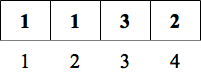
\includegraphics[width=0.3\textwidth]{img/assignment-encoding}
    \caption{An example of the assignment encoding for $n$ = 4 and $m$ = 3}\label{fig:assignment-encoding}
  \end{center}
\end{figure}

An encoding based on the centroids description is also considered in order to make the proposed crossover and mutation operations practicable. A centroids encoding defines a solution through the feature vectors existing in each centroid, being a matrix $C$ of size $m \times d$, where $m$ is the number of centroids (clusters) and $d$ is the number of features (see figure \ref{fig:centroids-encoding}). Thus, an entry $c_{ij}$ of $C$ corresponds to the value of the $j$-th feature of the $i$-th centroid ($i$ = 1 ... $m$; $j$ = 1 ... $d$).


\begin{figure}[h]
  \begin{center}
    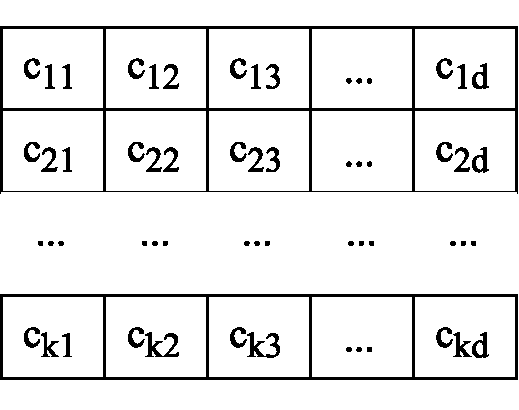
\includegraphics[width=0.3\textwidth]{img/centroids-encoding}
    \caption{The encoding based on centroids features}\label{fig:centroids-encoding}
  \end{center}
\end{figure}

%An encoding based on the centroids description is also considered in order to treat the redundancy that may arise from the object-cluster representation. For instance, the solutions (1,1,3,2) and (3,3,1,2) may be considered different solutions according to the object-cluster assignment, even though they are exactly the same solution. Thus, a centroids encoding is used to represent solutions whenever this redundancy must be detected, for example, when performing the crossover.

\begin{algorithm}[H]
\caption{Genetic algorithm framework}
\label{genetic-algo}
\begin{algorithmic}[1]
\STATE Initialize population
\WHILE{number of iterations without improvement $< itNoImprovement$}
\STATE Select parents $p_1$ and $p_2$
\STATE Generate an offspring $\theta$ from $p_1$ and $p_2$ (crossover)
\STATE Generate an individual $\theta'$ by mutating $\theta$ (mutation)
\STATE Apply local search on $\theta'$
\STATE Add $\theta$ and $\theta'$ to the population
\IF{population size is equal to the maximum size $\eta$ of population}
\STATE Select survivors
\IF{best solution not improved for $I$ iterations}
\STATE Diversify population
\ENDIF
\ENDIF
\ENDWHILE
\STATE Return best solution
\end{algorithmic}
\end{algorithm}

\section{Initial population}
The first step in a GA is the generation of an initial population. It has been recognized that if the initial population of the GA is good, then the algorithm has a better possibility of finding a good solution \cite{Burke2004, Zitzler2000}. Some factors can influence the initial population or should be taken into account when an initial population is generated randomly: the search space, the fitness function, the diversity, and the number of individuals \cite{DiazGomez2007}.

In this work, the initial population is randomly generated, by assigning each object to a cluster according to a discrete uniform distribution, i.e., where each outcome is equally likely to happen. To compose the initial population, $\mu$ individuals are created. Then, each initial individual is submitted to the local search.

\section{Individuals management}
In order to increase the population and start the competitive process of evolution we need to keep introducing new individuals. The generation of a new individual (offspring) begins with the random selection of two parents, $p_1$ and $p_2$, which are submitted to a crossover procedure that generates a child individual $\theta$. Then, $\theta$ is added to the population. As highly fit solutions have more chances to be selected for reproduction, the offspring -- which combines characteristics from each parent -- is likely to have a good fitness. Thus, we also consider the mutation operator, which generates a new individual $\theta'$ that is similar to $\theta$ and tends to be good regarding the fitness.

\subsection{Selection}
The selection is the stage where individuals from the population are chosen to mate and generate a new individual. Due to the evolutionary behaviour of GA, the most likely individuals to be chosen for selection are the ones with good fitness. That way, the good genes can be propagated to generate good children solutions. In the proposed method, the parent selection is done through a binary tournament, which randomly selects $w$ individuals (with uniform probability) from the population and keeps the one with the best fitness among the $w$ individuals to set the first parent. The fitness here considered is the value of the objective function (cost) of a solution. Then, the same selection scheme is performed to set the second parent.

\subsection{Crossover}
[Add image]

Once parent solutions $p_1$ and $p_2$ were selected, they should be submitted to a crossover procedure in order to produce a offspring (child) solution from them:

\begin{enumerate}
	\item Firstly, the minimum bipartite matching between centroids of $p_1$ and $p_2$ is calculated. One set of nodes in the matching problem is composed by the centroids of $p_1$ and the other set is composed by the centroids of $p_2$. The goal is to produce the one-to-one assignment of centroids from different sets, in such a way that the overall edges weight (distances) is minimized. This matching problem is solved by the Hungarian method \cite{Kuhn1955} and leads to $m$ pairs of centroids, where $m$ is the number of clusters (centroids).

	\item For each pair of centroids resulted from the minimum bipartite matching solution, one of them is randomly selected and set as a centroid of the offspring solution.

	\item Finally, data points are assigned to the closest offspring centroid.
\end{enumerate}

\subsection{Mutation}
[Add image]

The mutation of a solution is done by a biased relocation of a centroid. This strategy proved effective as it introduces some drastic movement in one centroid position, allowing the overall solution to have considerable changes that are not achieved by the local improvement. The following items describe how the mutation works:

\begin{enumerate}

	\item Randomly select a centroid $c^{*}$ and remove it from the solution.
	
	\item Among the $m-1$ remaining centroids, re-assign each data point to the closest centroid.
	
	\item Randomly select the position of a data point $x_i$ and re-insert $c^{*}$ in the position of $x_i$. This position is selected as in a wheel roulette, such that data points far from their current centroids are more likely to be chosen.
	
	\item Among the $m$ resulting centroids, re-assign each data point to the closest centroid.
		
\end{enumerate}

The mutation, in addition to generating a solution that is similar to the offspring -- which is typically a good solution due to elitism in parental selection -- also contributes significantly to the population diversity through the biased relocation of one centroid.

\subsection{Local improvement}
After the generation process done by crossover and mutation, $\theta$ is improved through a local search procedure. The local search aims to find a local optimum by applying local changes to the current solution. Here, the adopted local search is one run of the k-means algorithm. The k-means starts with the initial solution $\theta'$ with $m$ centroids $c_1$, $c_2$, ..., $c_m$, and proceeds by alternating between two steps:

\begin{enumerate}

	\item Assignment step: Assign each data point $x_i$ to the closest cluster $S_{k^{*}}$.
	
	\begin{equation}
	S_{k^{*}}^{(t)} = \{ x_i: \left \| c_{k^{*}}^{(t)} - x_i \right \| \leq  \left \| c_{j}^{(t)} - x_i \right \|, \quad j = 1, ..., m \}
	\end{equation}
	
	\item Update step: Calculate the new centroids $c_j$ to be the mean (average) point of the data points in the new clusters.
	
	\begin{equation}
	c_{j}^{(t+1)} = \frac{1}{\left | S_{j}^{(t)} \right |} \sum_{x_i \in S_{j}^{(t)}} x_i, \quad j = 1, ..., m
	\end{equation}
		
\end{enumerate}

Then the algorithm keeps repeating these two steps until the assignments no longer change, converging to a local optimum.

In our experiments, we use the k-means implementation of Greg Hamerly \cite{Hamerly2010}, who proposed an acceleration that gives the same answer of the standard Lloyd's k-means \cite{Lloyd1982} but is much faster in practice. This implementation avoids distance computations by using the triangle inequality and lower bounds on distances. The time per k-means iteration of the algorithm is O($nmd$+$md^2$), where $n$ is the number of data points, $m$ is the number of clusters and $d$ is the number of data dimensions (features). However, the calculated lower bounds allow to eliminate the innermost k-means loop in around 80\% of the time, which in practise is much faster than the standard k-means.

\section{Population management and termination}
One of the main challenges in population-based algorithms is avoiding premature convergence of the population. The selection of parents based on elitism tends to favour good individuals to mate, reducing the diversity of the genetic material in the coming generations of the population. In order to overcome this issue, we propose two mechanisms that preserve the good solutions and ensure the diversity. Thus, the search procedure can be lead to unexplored regions of the search space without losing promising individuals.

We call these mechanisms to complement the selection, crossover and local improvement operators \textit{Survivors selection} and \textit{Diversification} management.

\subsection{Survivors selection}
The \textit{Survivors selection} aims to select the best individuals to propagate when the maximum population size $\eta$ is achieved. This procedure determines the $\mu$ individuals that will go on to the next generation, by discarding $\lambda$ individuals ($\lambda = \eta - \mu$) that are either clones or bad regarding the fitness, according to algorithm \ref{survivors}.

This characteristic of eliminating clones and poor solutions reveals two aspects of the \textit{Survivors selection} mechanism. The first one is that population diversity is somehow maintained, as we favour the removal of clones first. The second is related to elitism, as the individuals with good fitness are preserved. Other aspects related to diversity can be observed in mutation and diversification operators.

\begin{algorithm}[H]
\caption{Survivors selection}
\label{survivors}
\begin{algorithmic}[1]
\FOR{$i = 1 ... \lambda$}
\STATE $X \leftarrow $ all individuals having a clone
\IF{$X \neq \emptyset$}
\STATE Remove $p \in X$ with maximum fitness
\ELSE
\STATE Remove $p$ in the population with maximum fitness
\ENDIF
\ENDFOR
\end{algorithmic}
\end{algorithm}

\subsection{Diversification management}
The \textit{Diversification} mechanism aims to ensure the genetic diversity in a population. It is actually a complementary procedure to diversify the population of solutions, once the mutation carries the most important role regarding this matter. \textit{Diversification} is called after the survivors selection whenever $I$ iterations happen without improving the best solution. It is performed by creating $\beta$ new individuals as in the initialization phase, i.e., individuals are randomly generated and then submitted to local search. As this process introduces a significant amount of new genetic material, it allows the exploration of unvisited regions of the search space.

\section{Computational complexity}